\section{Empirical Motivation: Concept Entanglement in Diffusion Models}
\label{subsec:motivation}

\begin{figure*}[htbp]
\centering

\setlength{\tabcolsep}{2pt}

\begin{tabular}{c c c c c}

 & \multicolumn{2}{c}{\textbf{Prompt with ``horse''}} & \multicolumn{2}{c}{\textbf{Prompt without ``horse''}} \\

 & Original & Unlearned & Original & Unlearned \\

\midrule

\textbf{ESD} &
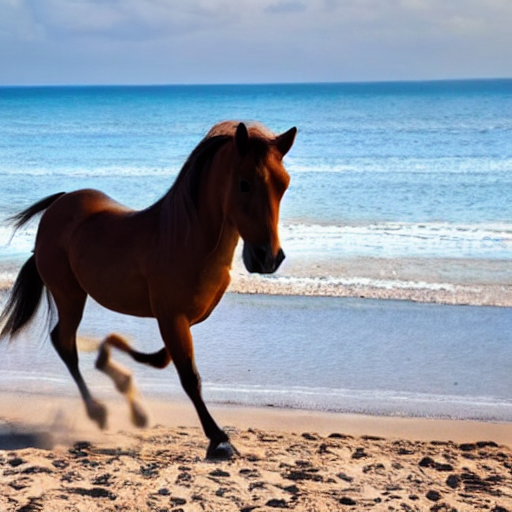
\includegraphics[width=0.22\linewidth]{img/esd_orig_horse.png} &
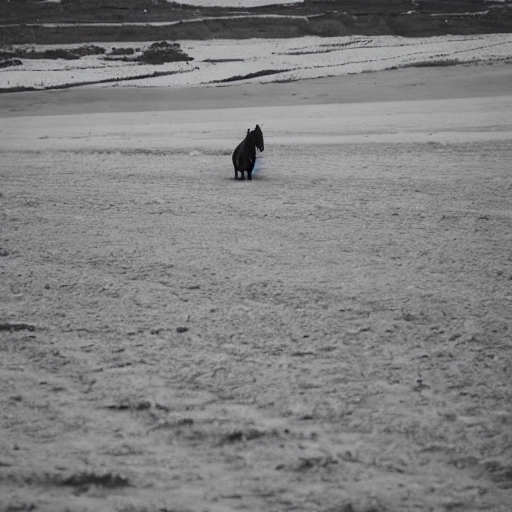
\includegraphics[width=0.22\linewidth]{img/esd_unlearn_horse.png} &
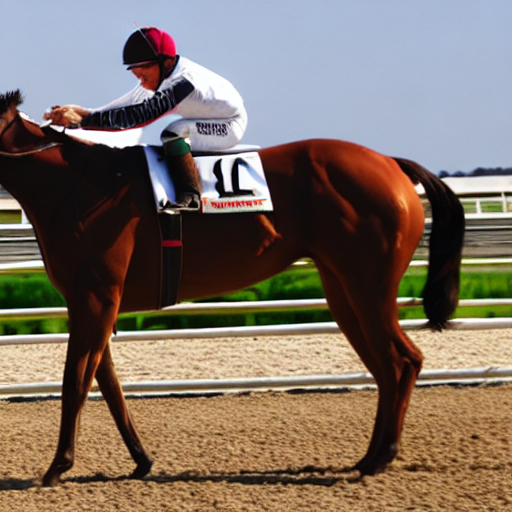
\includegraphics[width=0.22\linewidth]{img/esd_orig_nohorse.png} &
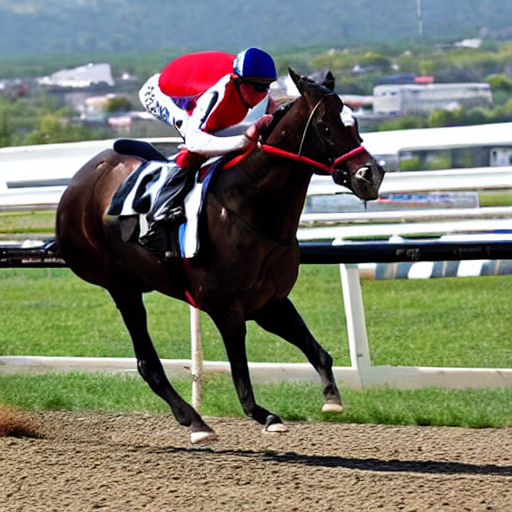
\includegraphics[width=0.22\linewidth]{img/esd_unlearn_nohorse.png} \\

\textbf{AdvUnlearn} &

\includegraphics[width=0.22\linewidth]{img/adv_orig_horse.png} &

\includegraphics[width=0.22\linewidth]{img/adv_unlearn_horse.png} &
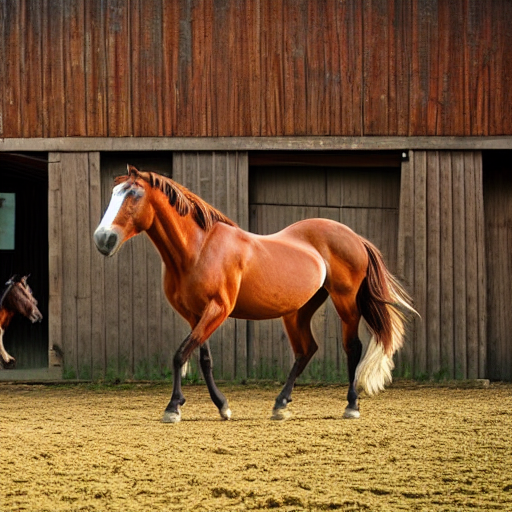
\includegraphics[width=0.22\linewidth]{img/adv_orig_nohorse.png} &
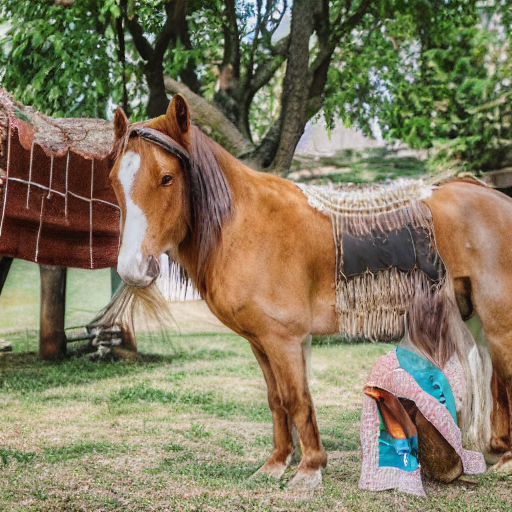
\includegraphics[width=0.22\linewidth]{img/adv_unlearn_nohorse.png} \\

\textbf{STEREO} &
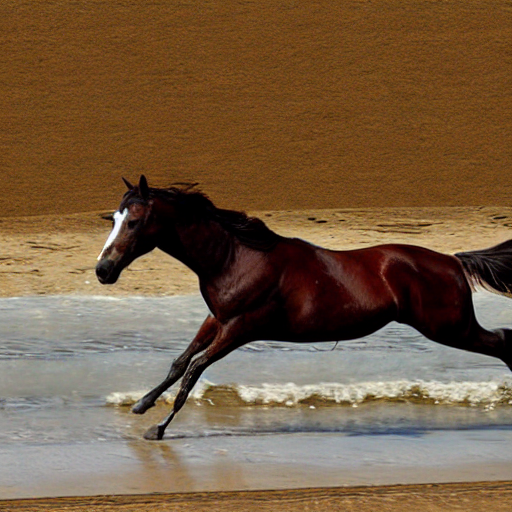
\includegraphics[width=0.22\linewidth]{img/stereo_orig_horse.png} &
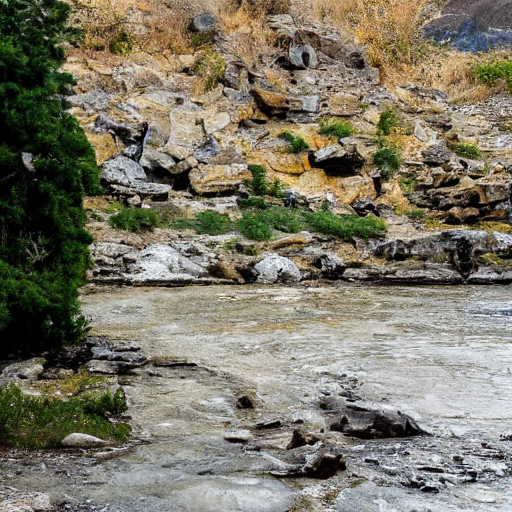
\includegraphics[width=0.22\linewidth]{img/stereo_unlearn_horse.png} &
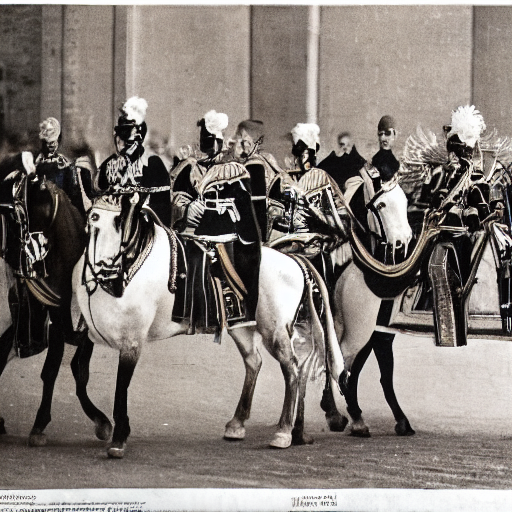
\includegraphics[width=0.22\linewidth]{img/stereo_orig_nohorse.png} &
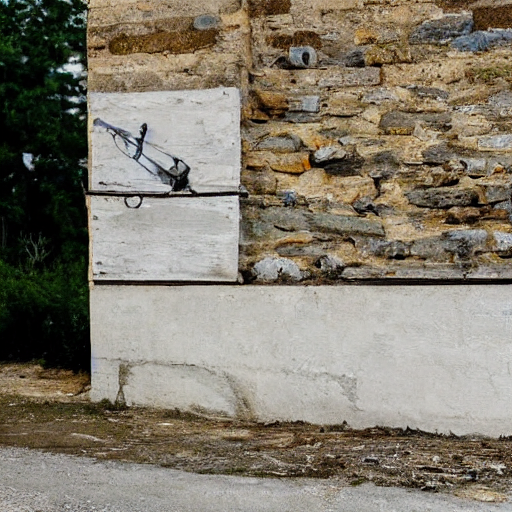
\includegraphics[width=0.22\linewidth]{img/stereo_unlearnnohorse.png} \\

\textbf{SaeUron} &
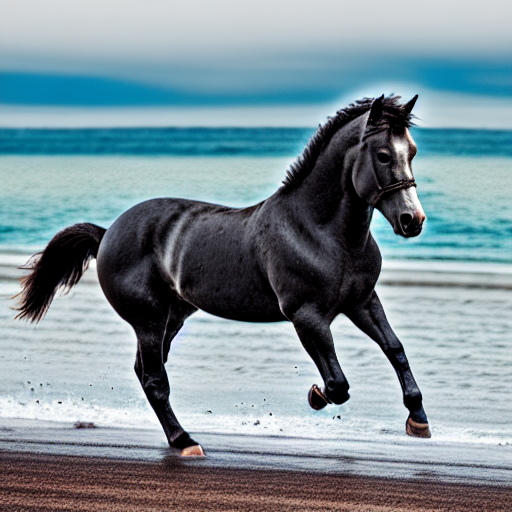
\includegraphics[width=0.22\linewidth]{img/saeuron_orig_horse.png} &
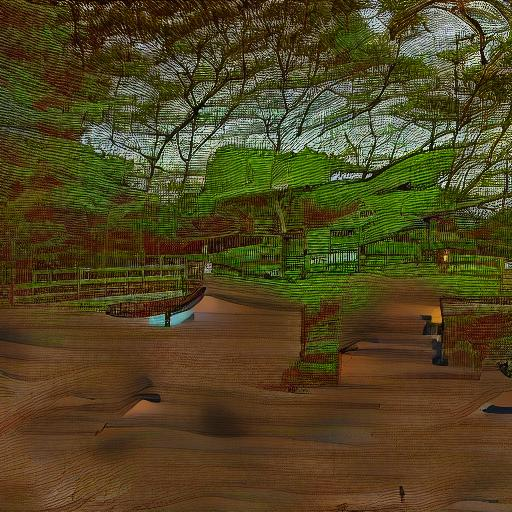
\includegraphics[width=0.22\linewidth]{img/saeuron_unlearn_horse.jpg} &
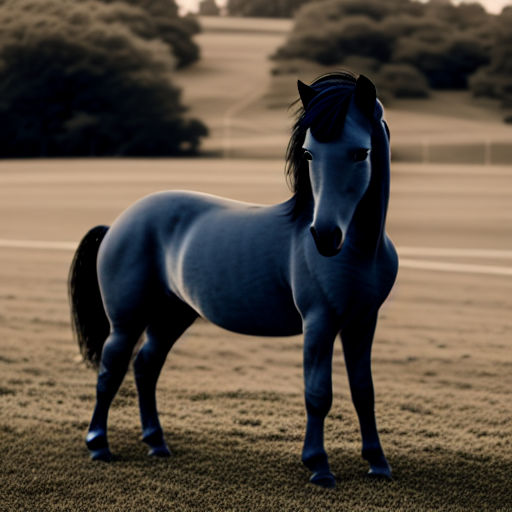
\includegraphics[width=0.22\linewidth]{img/saeuron_orig_nohorse.png} &
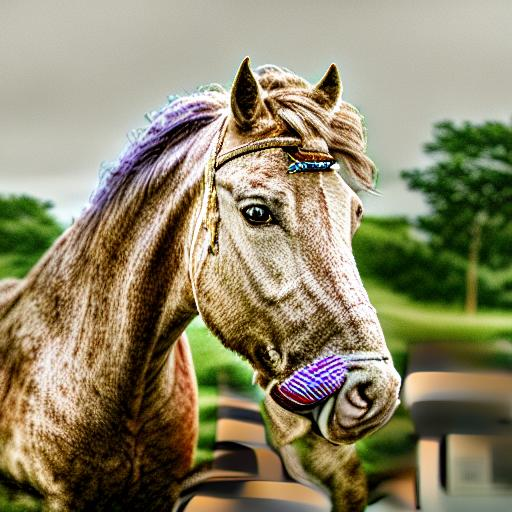
\includegraphics[width=0.22\linewidth]{img/saeuron_unlearn_nohorse.jpg} \\

\end{tabular}

\caption{
Empirical evidence of contextual concept leakage in diffusion unlearning.
Each row corresponds to a different unlearning method.
For prompts explicitly containing the token ``horse'' (left group), most unlearning methods suppress the concept in the generated image.
However, when the prompt omits the token but includes semantically related context (right group), the unlearned models frequently regenerate horses.
This behavior indicates that the concept is encoded through distributed contextual tokens rather than a single lexical trigger.
}

\label{fig:concept_leakage}
\end{figure*}

Existing diffusion unlearning methods typically assume that visual concepts are represented in a compositional and token-aligned manner within the model's text--image representation space. Under this assumption, removing a target concept token (e.g., ``horse'') should prevent the model from generating images containing that concept. 

In this section, we present empirical evidence that challenges this assumption. We demonstrate that diffusion models exhibit strong \textit{concept entanglement}: semantic concepts are distributed across correlated context tokens rather than tied to a single word. As a result, removing a concept token does not guarantee the removal of the underlying visual concept. These findings mirror observations from prior work~\cite{yuksekgonul2022and} showing that vision language models (VLMs) often behave like bag-of-words systems with weak sensitivity to token composition and relational structure.

\subsection{Prompt-Level Concept Leakage}

We first investigate whether diffusion models can regenerate an unlearned concept through contextual prompts that do not explicitly contain the target token.

We apply several recent concept erasure methods to remove the concept ``horse'' from a pretrained diffusion model. After unlearning, we construct prompts that omit the token ``horse'' but contain semantically related contextual descriptions, such as:

\begin{itemize}
\item ``a horse running on the beach''
\item ``Image of the animal a jockey rides at the racetrack''
\item ``Image of a pony in a country fair''
\item ``A royal procession with decorated ceremonial mounts''
% \item ``a cowboy jumping over a fence''
% \item ``person riding through a ranch field''
\end{itemize}

Despite the absence of the target token, the unlearned models frequently generate images containing horses. This behavior suggests that the model does not represent the concept ``horse'' as an isolated token-level feature. Instead, the concept emerges from the co-occurrence of multiple correlated tokens that collectively encode the underlying visual concept.

This phenomenon is consistent with prior findings that text encoders in multimodal models often approximate bag-of-words representations, where semantic information is distributed across tokens rather than tied to compositional structures.

\subsection{Utility Degradation on Neighbor Concepts}

\ali{i think this could be presented in a more general sense as an existing trade-off between susseptibility to the bad-of-words attack and utility degradation, which itself is due to the way the models are trained. Putting them in separate sections does not convey this connection.}

Next, we analyze the behavior of more robust unlearning methods designed to defend against adversarial prompts.

Methods such as STEREO aim to improve robustness by incorporating adversarial training during concept erasure. While these methods significantly reduce direct regeneration of the erased concept, we observe a different failure mode: degradation in the generation of semantically related concepts.

For example, after removing the concept ``horse'', models trained with robust erasure methods frequently fail to generate images containing nearby animal concepts such as ``deer''. Prompts such as:

\begin{itemize}
\item ``a deer standing in a forest''
\item ``a herd of deer grazing in a field''
\end{itemize}

often produce distorted or incorrect outputs.

This observation suggests that the representations of semantically related concepts occupy overlapping regions in the model's latent space. Consequently, removing one concept can inadvertently damage neighboring concepts, revealing the entangled structure of the underlying representation.

\subsection{Text-In-Image Prompt Injection Attack}

\ali{I think in the more general presentation of the trade-off, this section could be merged with section 3.1? But is this a good fit to the general scheme?}

Finally, we explore a prompt injection attack inspired by recent work showing that generative models can embed textual content directly into generated images.

We first generate images using the original (non-unlearned) model with prompts that explicitly reference the target concept, for example:

\begin{quote}
``two cowboys talking about a horse, with subtitles''
\end{quote}

The generated images often contain visible textual elements describing the concept. We then extract the text from these images using an OCR system and use the extracted text as a new prompt for the unlearned model.

Surprisingly, these prompts frequently cause the unlearned model to regenerate images containing horses, even though the original concept token is not explicitly provided as a prompt input.

This attack demonstrates a previously underexplored vulnerability of diffusion unlearning systems: concept reactivation through indirect textual signals embedded in generated content. The success of this attack further supports the hypothesis that concept representations are distributed across multiple correlated tokens and contexts rather than localized to individual words.

\subsection{Implications}

Together, these experiments provide strong evidence that diffusion models encode visual concepts through distributed contextual representations. As a result, token-level unlearning objectives are insufficient to guarantee concept-level deletion. These findings motivate the need for unlearning frameworks that reason about concept structure and contextual correlations rather than individual tokens.

\subsection{Bag-of-Words Concept Entanglement}
\varun{i think this should be a motivating experiment section? and highlight how earlier phenomenon were shown for VLMs but now you see this for diffusion too}

\varun{and before this, you want to present an analysis on the captions used in the training of these models based on the pos tagging stuff we have discussed a while ago}

Prior work on vision–language models (VLMs)~\cite{radford2021learning} has shown that text encoders
often fail to encode prompts compositionally. Instead, prompt embeddings
can frequently be approximated by a bag-of-words aggregation over token
embeddings~\cite{yuksekgonul2022and}. Under such representations, semantic
meaning arises from the co-occurrence of multiple tokens rather than the
presence of a single lexical trigger.

This observation is particularly relevant for diffusion models, which
reuse pretrained VLM-style text encoders to produce prompt embeddings
that condition image generation. Training captions in large-scale
text-to-image datasets exhibit strong co-occurrence patterns between
objects, actions, and scene descriptors. For example, captions
containing the concept \texttt{horse} often include tokens such as
\textit{rider}, \textit{saddle}, \textit{cowboy}, or \textit{stable}.
These contextual tokens form correlated patterns that frequently appear
together in training captions.

If the text encoder behaves approximately as a bag-of-words model,

\[
f_t(p) \approx \sum_{t \in p} \phi(t),
\]

then prompts containing only contextual tokens may produce embeddings
similar to those generated by prompts that explicitly include the
concept token. Formally, let $t_c$ denote a token associated with a
target concept $c$, and let $S_c$ denote a set of tokens that frequently
co-occur with $t_c$. Under a bag-of-words representation,

\[
\mathbb{E}[\mathbf{e}_p \mid t_c \in p]
\approx
\mathbb{E}[\mathbf{e}_p \mid S_c \subseteq p].
\]

This suggests that visual concepts may be encoded as distributed
patterns across multiple correlated tokens rather than isolated
lexical units. Consequently, removing the explicit concept token
does not necessarily eliminate the underlying visual concept if
sufficient contextual cues remain present.